\documentclass{standalone}
\usepackage{pgfplots}
\pgfplotsset{compat=1.18}

\begin{document}
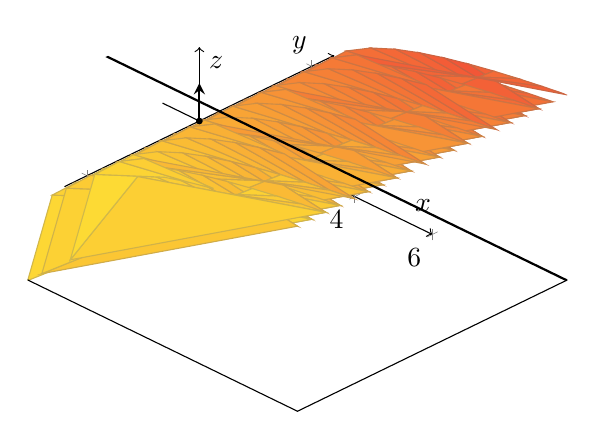
\begin{tikzpicture}
    \begin{axis}[
        view={45}{45},
        domain=-6:6,
        y domain=-6:6,
        colormap={grad}{color(0cm)=(yellow!80!white); color(3cm)=(red!80!white)},
        axis lines=middle,
        axis line style={->},
        xlabel=$x$,
        ylabel=$y$,
        zlabel=$z$,
        enlargelimits=false,
        samples=20,
        no markers,
        ]
        \addplot3 [
            surf,
            shader=faceted,
            point meta=x + y
        ] {ln(x + 1)};
        \draw [thick] (axis cs:-6,-6) -- (axis cs:6,-6);
        \draw [thick] (axis cs:-6,6) -- (axis cs:6,6);
        \draw [thick] (axis cs:6,-6) -- (axis cs:6,6);
        \filldraw [black] (axis cs:0,0,0) circle (1pt);
        \draw [-stealth, thick] (axis cs:0,0,0) -- (axis cs:0,0,1);
    \end{axis}
\end{tikzpicture}
\end{document}